\documentclass[11pt]{article}
\usepackage[margin=0.85in]{geometry}
\usepackage{listings}
\usepackage{xcolor}
\usepackage{parskip}
\usepackage{graphicx}
\usepackage{caption}
\usepackage{subcaption}

\lstset{
  basicstyle=\ttfamily\footnotesize,
  breaklines=true,
  language=Python,
  keywordstyle=\color{blue!70!black},
  commentstyle=\color{green!50!black},
  stringstyle=\color{red!70!black},
  showstringspaces=false,
  xleftmargin=10pt,
  aboveskip=4pt,
  belowskip=4pt,
}

\title{\vspace{-3em}EAS 5850 Homework 2: Report}
\author{Pennkey: delemos1}
\date{}

\begin{document}
\maketitle
\vspace{-2.5em}

\section*{1. Approach}
The script talks to the local Orthanc instance through \texttt{pyorthanc}'s REST client at \texttt{http://localhost:8042}. Part~2 calls \texttt{pyorthanc.find\_patients(query=\{"PatientID": "A034518"\})} to locate the CT study, then walks the patient/study/series/instance tree exposed by pyorthanc's resource wrappers. Series and instances are sorted by their DICOM \texttt{SeriesNumber} and \texttt{InstanceNumber} tags so ``series 4'' and ``image 130'' refer to clinically meaningful numbering rather than arbitrary list order. The target instance is loaded as a pydicom \texttt{Dataset} via \texttt{instance.get\_pydicom()}; header tags are read with \texttt{getattr}, pixel statistics are computed from \texttt{ds.pixel\_array.min()/max()/mean()}, and the results are written to \texttt{study\_info.json}. Part~3 queries for patient ID \texttt{3142537564}, iterates every instance in the study, mutates the seven required fields on the in-memory dataset, serializes back to bytes with \texttt{ds.save\_as(buf, enforce\_file\_format=True)}, uploads each modified instance via \texttt{client.post\_instances(buf.getvalue())}, and finally deletes the original study with \texttt{client.delete\_studies\_id(original\_study\_id)} so only the modified version remains on the server.

\section*{2. How DICOM Differs from Other Image Formats}
A DICOM instance is not a bare pixel grid: it is a structured object built from typed tags. Every element carries a Value Representation (VR) that governs its on-wire format. Dates use VR \texttt{DA} as \texttt{YYYYMMDD} strings, person names use \texttt{PN} in \texttt{Family\^{}Given\^{}Middle} order, UIDs are dotted decimal strings, and pixel data is a binary blob whose layout depends on the chosen transfer syntax. Unlike PNG or JPEG, identity is not file-based --- studies, series, and instances are linked by persistent UIDs (\texttt{StudyInstanceUID}, \texttt{SeriesInstanceUID}, \texttt{SOPInstanceUID}) that are part of the dataset itself. Patient demographics, acquisition geometry, and equipment manufacturer live alongside the pixels rather than in a sidecar EXIF block, and any modification to a key tag (such as \texttt{StudyInstanceUID}) effectively re-identifies the object.

\section*{3. Accommodations}
The assignment limits imports to \texttt{pyorthanc} and \texttt{json} (plus \texttt{numpy} if needed). My script never imports \texttt{pydicom} directly --- it uses \texttt{instance.get\_pydicom()}, which returns a \texttt{Dataset} whose own \texttt{save\_as} method handles serialization. Modified values were formatted to DICOM VR conventions: birth date as \texttt{"19780101"} rather than \texttt{"1/1/1978"}, the physician name as \texttt{"Spock\^{}Thomas"}, and the new \texttt{StudyInstanceUID} as a bare dotted string. Series and instance selection use DICOM-assigned numbers via \texttt{sorted(..., key=\_series\_number)} so the ordering matches what a radiologist sees. Pixel statistics are cast with \texttt{int()} / \texttt{float()} to convert NumPy scalars into JSON-serializable Python numerics.

\section*{4. Hardest Errors}
The hardest parts of this exercise were not the algorithmic ones but the upstream work: familiarizing myself with the DICOM data model, getting reliable access to it through Orthanc, and finding the right Python packages to drive both. Initially I wasted time trying to compute the patient's age from \texttt{PatientBirthDate} before realizing the assignment's hint (``found as a string'') was pointing at the \texttt{PatientAge} tag in \texttt{045Y} format. I also tried fictional class names like \texttt{pyorthanc.OrthancClient}, when the actual entry point is \texttt{pyorthanc.Orthanc} for the low-level client and \texttt{pyorthanc.find\_patients(...)} for the high-level resource wrappers. The Orthanc web UI was indispensable for grounding all of this --- once I could visually confirm what was loaded (Figure~\ref{fig:orthanc}) and view the pixels in a 3D viewer (Figure~\ref{fig:volview}), it was much easier to write code that matched what was actually on disk.

The single most concrete error came at the end of Part~3. Uploading the modified DICOM bytes does \emph{not} replace the original study on Orthanc --- because changing \texttt{StudyInstanceUID} mints a brand new study identity, both the old (patient \texttt{3142537564}) and the new (patient \texttt{8675309}) ended up coexisting on the server. A verification query for the old patient ID still returned a match even after my modification loop ran, which would silently fail the autograder. My initial code:

\begin{lstlisting}
for series in study.series:
    for instance in series.instances:
        ds = instance.get_pydicom()
        ds.PatientID = "8675309"
        # ... (other six field changes) ...
        buf = io.BytesIO()
        ds.save_as(buf, enforce_file_format=True)
        client.post_instances(buf.getvalue())
# Result: two studies on Orthanc, original still present.
\end{lstlisting}

The fix was to capture the original Orthanc study ID before iterating and delete it once all modified instances had been uploaded:

\begin{lstlisting}
study = patient.studies[0]
original_study_id = study.id_
for series in study.series:
    for instance in series.instances:
        ds = instance.get_pydicom()
        ds.StudyInstanceUID       = "1.2.840.20252025"
        ds.AccessionNumber        = "EAS5850-12345678"
        ds.PatientBirthDate       = "19780101"
        ds.PatientSex             = "O"
        ds.StudyDate              = "20221231"
        ds.PatientID              = "8675309"
        ds.ReferringPhysicianName = "Spock^Thomas"
        buf = io.BytesIO()
        ds.save_as(buf, enforce_file_format=True)
        client.post_instances(buf.getvalue())
client.delete_studies_id(original_study_id)
\end{lstlisting}

After this change, querying Orthanc for patient \texttt{3142537564} returned zero matches and querying for patient \texttt{8675309} returned one patient whose study had all seven fields set to the expected values.

\section*{Appendix: Proof of Access}

\begin{figure}[h!]
  \centering
  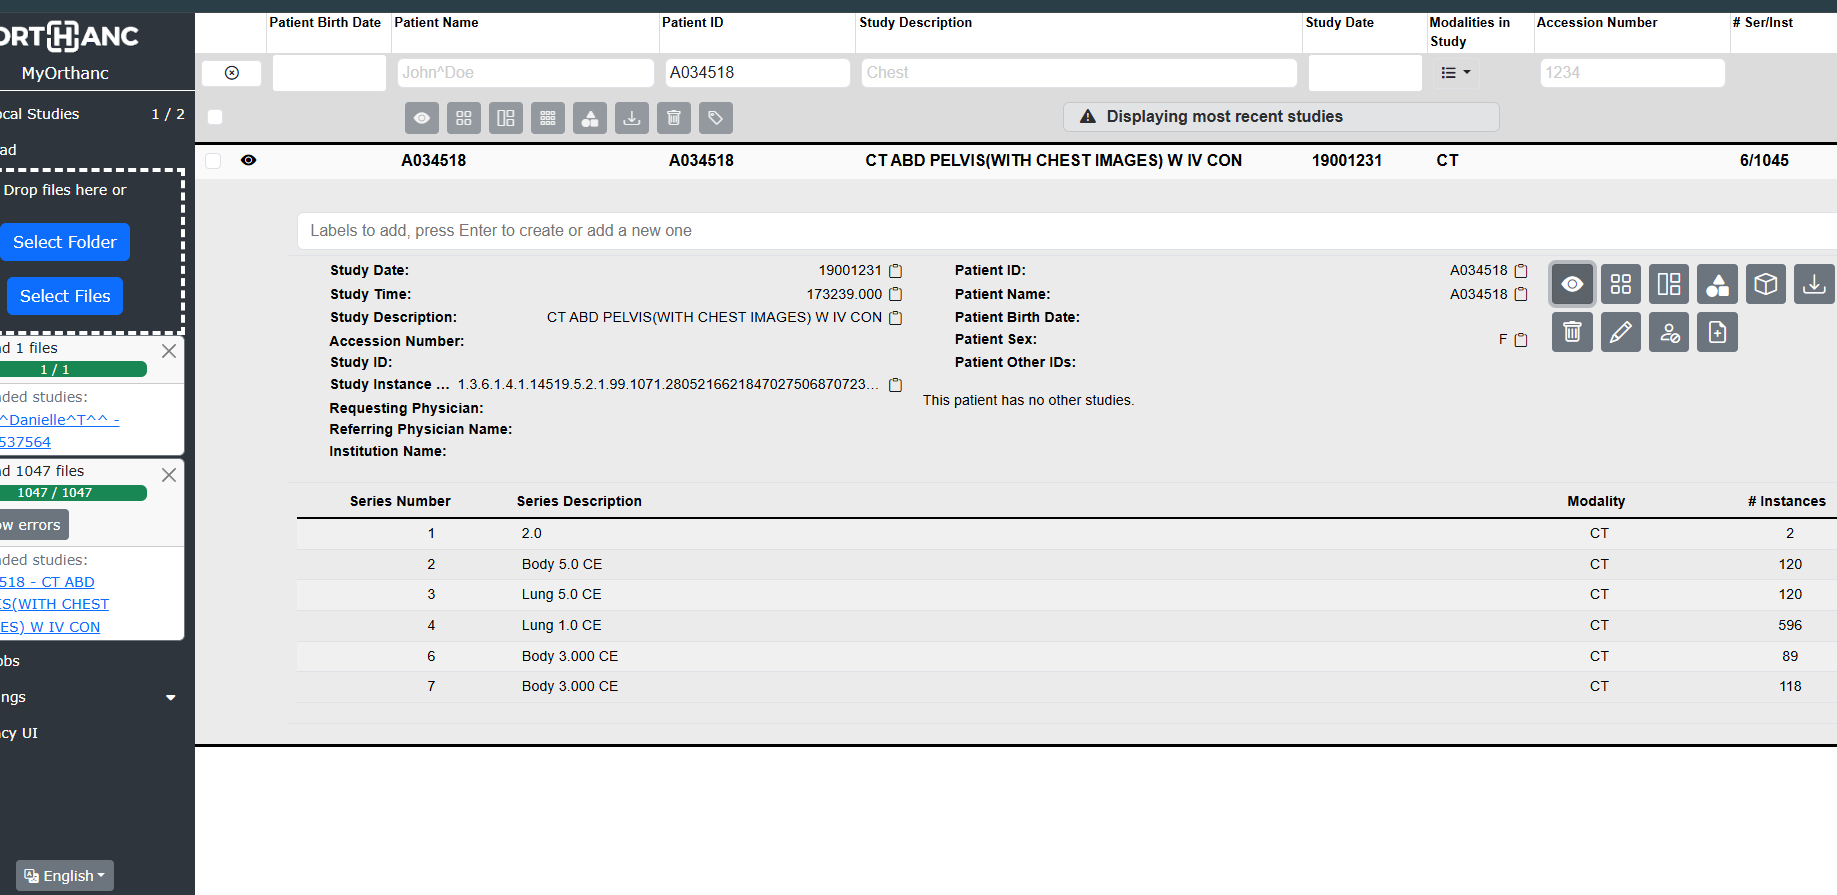
\includegraphics[width=0.95\textwidth]{orthanc.png}
  \caption{The uploaded \texttt{CT ABD PELVIS(WITH CHEST IMAGES) W IV CON} study for patient \texttt{A034518} in the Orthanc web UI, showing all six CT series indexed under one study.}
  \label{fig:orthanc}
\end{figure}

\begin{figure}[h!]
  \centering
  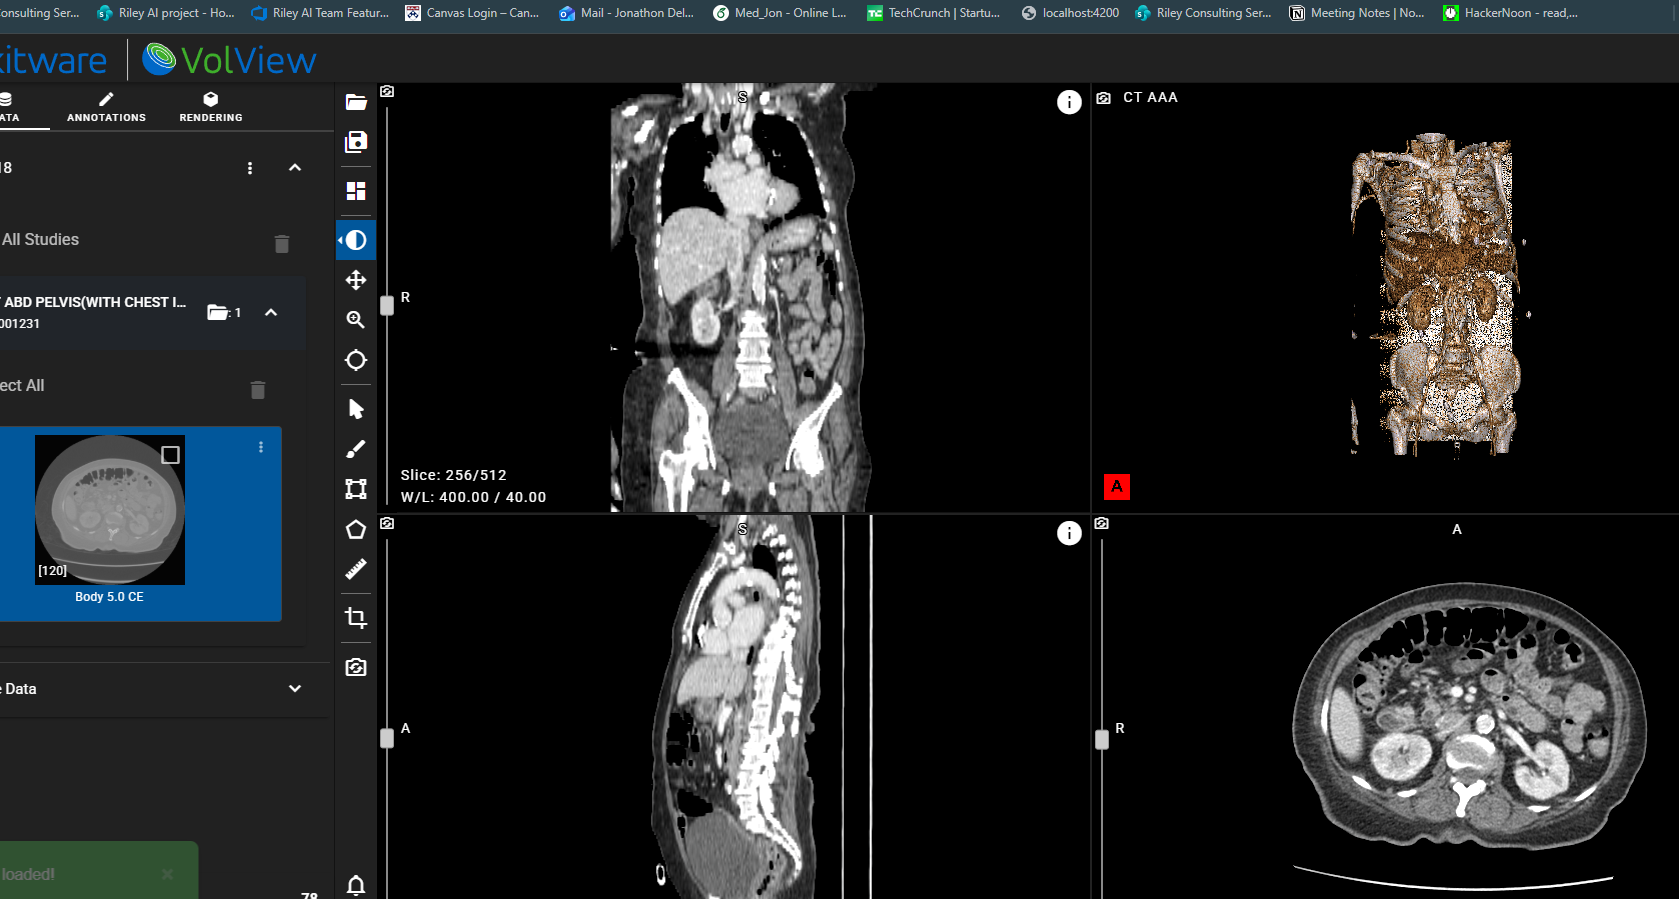
\includegraphics[width=0.85\textwidth]{orthanc2.png}
  \caption{Pixel data for the same study rendered in VolView, confirming that the DICOM files retrieved from Orthanc decode correctly and the pixel array values used in Part~2 are valid.}
  \label{fig:volview}
\end{figure}

\end{document}
